\levelstay{Problem 3.3.3 (AO)}

Instead of the very specific decaying exponential form in problem 3.2, suppose you are given only that
\begin{itemize}
\item[(i)] $\overline{\eta(t_1) \eta(t_2)}$ is a function of $|t_1-t_2|$, the magnitude of the 
time difference between the two time arguments
\item[(ii)] $\overline{\eta(t_1) \eta(t_2)}$ tends to zero as $|t_1-t_2|\rightarrow\infty$.
\end{itemize}
\textbf{Goal:} Show that the inescapable conclusion based on properties (i) and (ii) is that $\overline{v^2(t)}$ increases linearly with $t$ at long times, in the absence of a damping term $\gamma$.

In what follows, we will denote the $\overline{\eta(t_1) \eta(t_2)}$ by $f(|t_1-t_2|)$. Notice that the argument of $f$ is identically zero $\forall~t_1=t_2$. Let us use this fact to break the integral below into two equal parts:
\begin{eqnarray}
(\overline{v^2(t)}-v_0^2) \times m^2 &=& \int_{0}^{t} dt_1 \int_{0}^{t} dt_2 ~ f(|t_1-t_2|) \nonumber \\
&=& \bigg\{\underbrace{\int_{0}^{t} dt_1 \int_{0}^{t_1} dt_2}_{=T_1} + \underbrace{\int_{0}^{t} dt_1 \int_{t_1}^{t} dt_2}_{=T_2} \bigg\} f(|t_1-t_2|)\label{eq:eq3p3},
\end{eqnarray}
where $T_1$ and $T_2$ correspond to the triangular-shaped integration domains shown in Fig. \ref{fig:3p3}. To show that these two integrals are equal, consider a displacement from the line $t_2=t_1$, given by $(t_1-\Delta t, t_1+\Delta t)$. Evaluating $f$ at this point yields $f(|-\Delta t-\Delta t|)=f(|2\Delta t|)$. Similarly, we can evaluate $f$ at the point $(t_1+\Delta t, t_1-\Delta t)$, which also yields $f(|+\Delta t+\Delta t|)=f(|2\Delta t|)$. Clearly then, the integrals over each of these domains are equal. To show this using calculus, let us reverse the order of integration in the second term in Eq. (\ref{eq:eq3p3}), which yields
\begin{eqnarray}
(\overline{v^2(t)}-v_0^2) \times m^2
&=& \bigg\{\underbrace{\int_{0}^{t} dt_1 \int_{0}^{t_1} dt_2}_{=T_1} + \underbrace{\int_{0}^{t} dt_2 \int_{0}^{t_2} dt_1}_{=T_2} \bigg\} f(|t_1-t_2|)  \nonumber \\
&=& 2 \int_{0}^{t} dt_1 \int_{0}^{t_1} dt_2 ~f(|t_1-t_2|).  \nonumber \\
\end{eqnarray}
The second line follows from the fact that we can interchange labels for $t_1$ and $t_2$ in the second integral, as these are just dummy variables. Now one has that
\begin{eqnarray}
(\overline{v^2(t)}-v_0^2) \times m^2 &=& 2 \int_{0}^{t} dt_1 \int_{t_1}^{0} -dt' ~f(|t'|)  \nonumber \\ 
&=& 2 \int_{0}^{t} dt_1 \int_{0}^{t_1} dt' ~f(|t'|)  \nonumber \\ 
&=& 2 \int_{0}^{t} dt'~f(|t'|) \int_{t'}^{t_1} dt_1  \nonumber \\ 
&=& 2 \int_{0}^{t} dt'~ (t-t')f(|t'|).
\end{eqnarray}
This result was obtained by substituting $t'=t_1-t_2$ and then reversing the order of integration for integrals over $dt_1$ and $dt'$. Assuming $f(|t'|)$ decays over some characteristic timescale $\tau$, for $t\gg \tau$ , we have that 
\begin{eqnarray}
(\overline{v^2(t)}-v_0^2) \times m^2 &=& 2 \int_{0}^{t} dt'~ (t-t')f(|t'|) \\
&=& 2 t \bigg( \int_{0}^{t} dt'~ f(|t'|) - \int_{0}^{t} dt'~ \frac{t'}{t} f(|t'|)\bigg)\\
& \simeq & 2t \int_{0}^{t} dt'~ f(|t'|),
\end{eqnarray}
as the second term is subdominate until $t'\sim t$, but then $f(|t'|) \rightarrow 0$ since $t'\sim t>>\tau$. As an example, consider $f(|t'|)=C \exp(t'/\tau)$. The integral above equates to $2C(t \tau - \tau^2)$.
\begin{figure}[h]
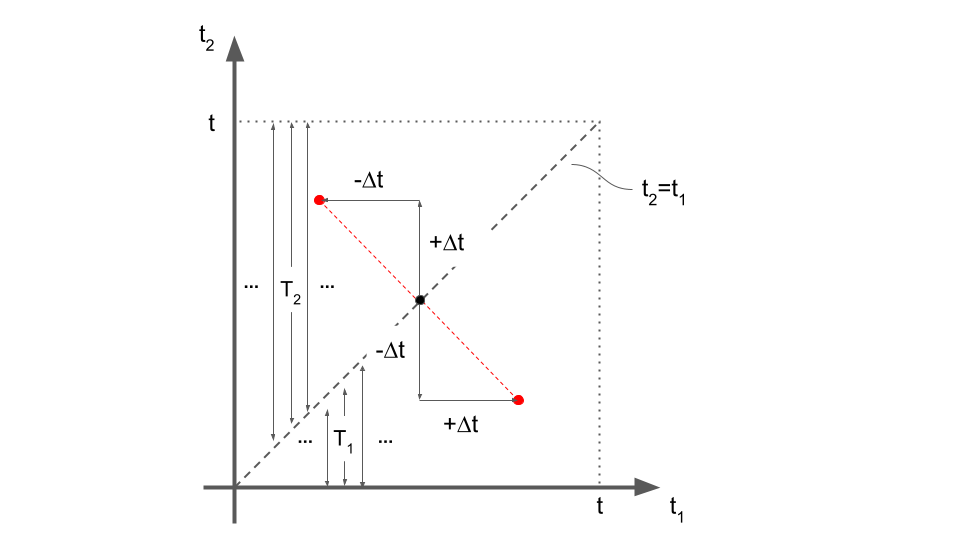
\includegraphics[width=16cm]{fig_problem_3p3.png}
    \caption{Symmetry of the integration domain for the integral $ \int_{0}^{t} dt_1 \int_{0}^{t} dt_2 ~ f(|t_1-t_2|)$.}
    \label{fig:3p3}
\end{figure}